\documentclass[10pt,a4paper]{article}
\usepackage[margin=0.72in]{geometry}
\usepackage{amsmath}
\usepackage{booktabs}
\usepackage{array}
\usepackage[table,dvipsnames]{xcolor}
\usepackage{fancyhdr}
\usepackage{hyperref}
\usepackage{microtype}
\usepackage{enumitem}
\usepackage{tikz}
\usepackage{pgfplots}
\pgfplotsset{compat=1.17}

\definecolor{navy}{HTML}{1F4E79}
\definecolor{lightblue}{HTML}{EAF2F8}
\hypersetup{colorlinks=true,linkcolor=navy,urlcolor=navy}
\setlength{\parindent}{0pt}
\setlength{\parskip}{5pt}
\setlength{\emergencystretch}{2em}
\setlist{nosep,leftmargin=1.3em}
\pagestyle{fancy}
\fancyhf{}
\lhead{ML Assignment 1: Polynomial Regression}
\rhead{BT2024128}
\cfoot{\thepage}
\renewcommand{\headrulewidth}{0.4pt}

\newcommand{\metric}[1]{\textcolor{navy}{\textbf{#1}}}

\begin{document}

\begin{center}
{\LARGE\bfseries Polynomial Regression for Geothermal Systems}\par\vspace{6pt}
{\large Machine Learning Assignment 1}\par\vspace{10pt}
\begin{tabular}{rl}
\textbf{Roll number:} & BT2024128 \\
\textbf{Problems:} & Steam turbine optimization (var1), thermal reservoir mapping (var2) \\
\textbf{Primary metrics:} & Mean Squared Error (MSE), coefficient of determination ($R^2$)
\end{tabular}
\par\vspace{5pt}{\small\textbf{GitHub repository:} \url{https://github.com/oki-dokii/ML-Assignment1_BT2024128}}
\end{center}

\section*{Abstract}
Two polynomial regression models were developed for the personalized datasets assigned to BT2024128. Feature subsets were screened with ordinary least squares (OLS), then regularized models were compared using cross-validation. The selected var1 model expands all six inputs to degree 5, uses Lasso to select terms, and refits them with Ridge; var2 expands all three inputs to degree 12 and uses Ridge alone. Repeated five-fold cross-validation produced MSE 0.2975 and $R^2=0.9724$ for var1, and MSE 0.2291 and $R^2=0.9945$ for var2.

\section{Dataset and task}
Each problem contains 1,000 training observations and 1,000 test observations. All columns are numeric, all input variables lie between $-1$ and $1$, and no values are missing. The training sets contain the continuous target $y$; the test targets are hidden.

\begin{table}[h]
\centering
\rowcolors{2}{lightblue}{white}
\begin{tabular}{lccc}
\toprule
Problem & Training shape & Test shape & Candidate inputs \\
\midrule
var1 & $1000 \times 7$ & $1000 \times 6$ & $x_1,\ldots,x_6$ \\
var2 & $1000 \times 4$ & $1000 \times 3$ & $x_1,x_2,x_3$ \\
\bottomrule
\end{tabular}
\end{table}

The train and test files for each problem were kept separate. Test values were used only after the final configuration had been selected and fitted on the complete corresponding training set.

\section{Polynomial regression pipeline}
For $p$ selected inputs and maximum degree $d$, the expansion contains every monomial whose total degree is at most $d$. Excluding the constant term, the number of generated terms is
\[
N(p,d)=\binom{p+d}{d}-1.
\]
The prediction model is linear in these expanded terms:
\[
\widehat{y}=\beta_0+\sum_{j=1}^{N(p,d)}\beta_j\phi_j(\mathbf{x}).
\]
Both scikit-learn pipelines apply \texttt{PolynomialFeatures}, then \texttt{StandardScaler}. Var1 next uses Lasso ($\alpha_L=0.03$) to retain terms with nonzero coefficients, then Ridge ($\alpha_R=0.1$) to refit those terms. Lasso minimizes squared error plus an $L_1$ coefficient penalty, encouraging sparse selection. Var2 uses Ridge alone ($\alpha_R=1$). The Ridge stage minimizes
\[
\sum_i\bigl(y_i-\beta_0-\mathbf{z}_i^\top\boldsymbol\beta\bigr)^2
+\alpha_R\lVert\boldsymbol\beta\rVert_2^2,
\]
where $\mathbf{z}_i$ contains the selected standardized polynomial terms. Ridge shrinks large coefficients and helps control variance. The intercept is not penalized. Expansion, scaling, and var1 term selection are all fitted inside each validation fold to prevent leakage.

\newpage\thispagestyle{fancy}
\section{Model-selection procedure}
The following procedure was applied independently to var1 and var2.

\begin{enumerate}
\item Screen every non-empty feature subset using OLS polynomial regression. Degrees up to 10 for var1 and 20 for var2 were considered, omitting OLS designs with more than 700 terms against 800 fitting observations per fold.
\item Keep the full feature sets because they had the lowest OLS validation error by a large margin.
\item Search Ridge models on these feature sets: degrees 3--6 and $\alpha_R\in\{0.1,1,3,10,30,100\}$ for var1; degrees 7--16 and $\alpha_R\in\{0.01,0.1,1,3,10\}$ for var2.
\item For var1 degree 5, also search Lasso term-selection strengths $\alpha_L\in\{0.003,0.01,0.03\}$ followed by Ridge strengths $\alpha_R\in\{0.1,1,10,30\}$. Keep var2 Ridge-only because tested Lasso selection did not lower its five-fold MSE.
\item Compare MSE (primary) and $R^2$ (secondary) using shuffled five-fold cross-validation. Check the var1 tuning procedure with a separate outer five-fold, inner three-fold nested validation.
\item Re-evaluate each fixed final configuration using five repeats of five-fold cross-validation.
\end{enumerate}

Ridge permits more polynomial terms than OLS because its penalty stabilizes coefficient estimation. Lasso removes weak or redundant degree-5 terms in var1. All shuffled folds use fixed seeds, and the test targets were never used for these decisions.

\subsection{Degree comparison}

\begin{table}[h]
\centering
\caption{Five-fold cross-validation of representative configurations}
\rowcolors{2}{lightblue}{white}
\begin{tabular}{llrrrr}
\toprule
Problem & Model & Degree & $\alpha_L$ & $\alpha_R$ & Mean MSE \\
\midrule
var1 & OLS & 4 & -- & 0 & 0.7725 \\
var1 & OLS & 5 & -- & 0 & 1.0671 \\
var1 & Ridge & 5 & -- & 10 & 0.4265 \\
var1 & Lasso + Ridge & 5 & 0.01 & 0.1 & 0.3235 \\
var1 & \textbf{Lasso + Ridge} & \textbf{5} & \textbf{0.03} & \textbf{0.1} & \textbf{0.3082} \\
\midrule
var2 & OLS & 8 & -- & 0 & 0.2544 \\
var2 & Ridge & 10 & -- & 1 & 0.2346 \\
var2 & \textbf{Ridge} & \textbf{12} & -- & \textbf{1} & \textbf{0.2268} \\
var2 & Ridge & 13 & -- & 1 & 0.2307 \\
\bottomrule
\end{tabular}
\end{table}

For var1, Lasso selection plus Ridge improves on Ridge alone at degree 5. The nested procedure averaged MSE 0.3086 and $R^2=0.9714$ across its outer folds; four of five inner searches chose $\alpha_L=0.03,\alpha_R=0.1$, while one chose $\alpha_R=1$. For var2, degree-12 Ridge remained best among the tested candidates.

\section{Feature selection}
The preliminary OLS screen favored all available inputs for both datasets. The best five-feature var1 alternative ($x_1,x_2,x_3,x_5,x_6$, degree 3) had MSE 1.8294, compared with 0.7725 for the full-feature degree-4 OLS baseline. All lower-dimensional var2 subsets were far behind the full three-feature degree-8 OLS model. Thus input variables were retained, while var1's Lasso stage selected among their expanded polynomial terms. It retained 69 of 461 terms after the final full-data fit.

\newpage\thispagestyle{fancy}
\section{Final validation results}

\begin{table}[h]
\centering
\caption{Repeated five-fold validation of the selected models (five repeats)}
\rowcolors{2}{lightblue}{white}
\begin{tabular}{lcccrr}
\toprule
Problem & Final model & Degree & Retained terms & MSE & $R^2$ \\
\midrule
var1 & Lasso + Ridge & 5 & 69 of 461 & $0.2975 \pm 0.0296$ & $0.9724 \pm 0.0036$ \\
var2 & Ridge & 12 & 454 & $0.2291 \pm 0.0251$ & $0.9945 \pm 0.0013$ \\
\bottomrule
\end{tabular}
\end{table}

The repeated estimates are close to the original five-fold screening scores, which shows that the choices are not tied to one random split. A separate five-fold out-of-fold prediction run gave the following results.

\begin{table}[h]
\centering
\rowcolors{2}{lightblue}{white}
\begin{tabular}{lrrrr}
\toprule
Problem & OOF MSE & OOF $R^2$ & Training MSE & Training $R^2$ \\
\midrule
var1 & 0.3082 & 0.9717 & 0.2360 & 0.9783 \\
var2 & 0.2268 & 0.9947 & 0.1487 & 0.9965 \\
\bottomrule
\end{tabular}
\end{table}

\subsection{Diagnostic interpretation}
For var1, out-of-fold predictions track the identity line across negative and positive scores. Residuals are centered near zero, with a few larger deviations at extreme responses. Selecting a sparse set of degree-5 terms reduced five-fold MSE from 0.4265 for Ridge-only to 0.3082. The 69-term count above comes from fitting all 1,000 labeled rows; each validation fold selected terms independently.

For var2, out-of-fold predictions lie close to the identity line over the observed target range, approximately $-30$ to $39$. Residuals remain centered around zero without a strong systematic curve. Degree 12 captures more structure than the earlier degree-8 OLS baseline while Ridge limits unstable coefficients.

\section{Final training and test inference}
After selection, each pipeline was refitted on all 1,000 observations from its training dataset. Predictions were generated in the original test-row order. The final output ranges were $-10.1324$ to $16.6722$ for var1 and $-29.7657$ to $38.7586$ for var2. Both submission files follow the provided sample: exactly 1,000 finite predictions in a single column named \texttt{y}, with no exported row index.

\clearpage
\section{Validation plots}
\thispagestyle{fancy}
The curves show five-fold validation MSE over the degrees tested for each model family. Lower values are better. These plots make the selected degrees and the effect of regularization visible beyond the representative configurations in Table 1.

\begin{center}
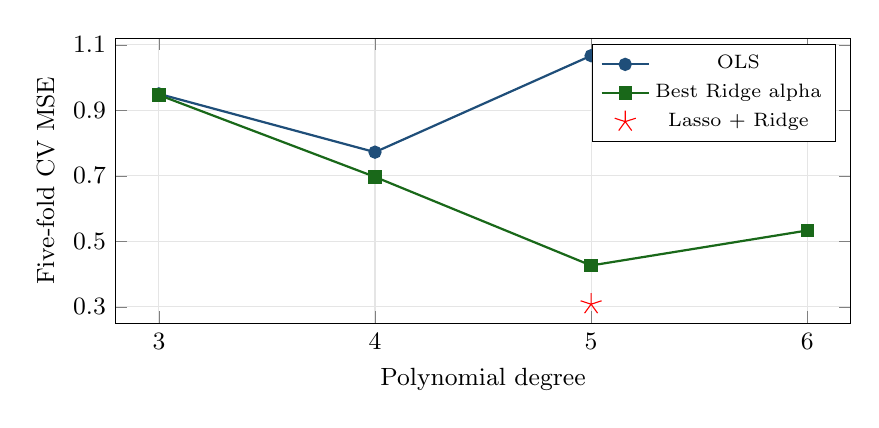
\begin{tikzpicture}
\begin{axis}[
  width=0.90\linewidth,height=5.2cm,
  xmin=2.8,xmax=6.2,ymin=0.25,ymax=1.12,
  xtick={3,4,5,6},ytick={0.3,0.5,0.7,0.9,1.1},
  xlabel={Polynomial degree},ylabel={Five-fold CV MSE},
  grid=major,grid style={gray!20},
  legend style={font=\scriptsize,at={(0.98,0.98)},anchor=north east},
  tick label style={font=\small},label style={font=\small}
]
\addplot[navy,thick,mark=*] coordinates {(3,0.950467) (4,0.772522) (5,1.067110)};
\addlegendentry{OLS}
\addplot[ForestGreen!75!black,thick,mark=square*] coordinates {(3,0.947073) (4,0.696954) (5,0.426465) (6,0.533301)};
\addlegendentry{Best Ridge alpha}
\addplot[Red,only marks,mark=star,mark size=4pt] coordinates {(5,0.308238)};
\addlegendentry{Lasso + Ridge}
\end{axis}
\end{tikzpicture}\\[2pt]
{\small\textbf{Figure 1.} var1: degree-5 Lasso selection followed by Ridge has the lowest tested MSE.}
\end{center}

For var2, the best Ridge penalty at each searched degree reaches its minimum at degree 12. Higher tested degrees do not improve the score.

\begin{center}
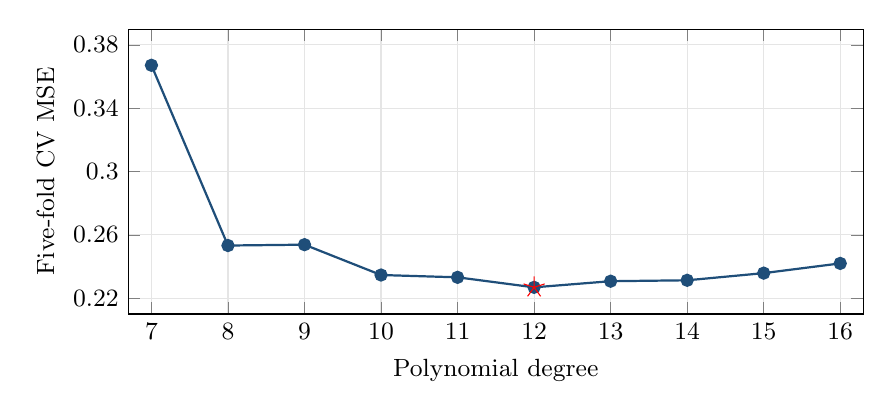
\begin{tikzpicture}
\begin{axis}[
  width=0.90\linewidth,height=5.2cm,
  xmin=6.7,xmax=16.3,ymin=0.21,ymax=0.39,
  xtick={7,8,9,10,11,12,13,14,15,16},
  ytick={0.22,0.26,0.30,0.34,0.38},
  xlabel={Polynomial degree},ylabel={Five-fold CV MSE},
  grid=major,grid style={gray!20},
  tick label style={font=\small},label style={font=\small}
]
\addplot[navy,thick,mark=*] coordinates {(7,0.367143) (8,0.253263) (9,0.253801) (10,0.234636) (11,0.233177) (12,0.226847) (13,0.230725) (14,0.231299) (15,0.235823) (16,0.241969)};
\addplot[Red,only marks,mark=star,mark size=4pt] coordinates {(12,0.226847)};
\end{axis}
\end{tikzpicture}\\[2pt]
{\small\textbf{Figure 2.} var2: degree-12 Ridge is the minimum within the searched range.}
\end{center}

Full-resolution \href{https://github.com/oki-dokii/ML-Assignment1_BT2024128/blob/main/plots/degree_selection.png}{degree-search} and \href{https://github.com/oki-dokii/ML-Assignment1_BT2024128/blob/main/plots/oof_diagnostics.png}{out-of-fold prediction and residual} plots can be viewed in the GitHub repository.

\clearpage
\section{Reproducibility and safeguards}
\thispagestyle{fancy}
The implementation provides separate scripts for selection and inference. The selection script writes OLS, Ridge, and Lasso-plus-Ridge search tables, nested and repeated-validation metrics, a degree-selection figure, and out-of-fold diagnostic plots. The prediction script validates schemas, rejects missing or nonnumeric values, checks prediction length and finiteness, saves the fitted pipelines, and writes the two submission CSV files.

\begin{itemize}
\item \textbf{No test leakage:} Neither test inputs nor hidden targets influence feature or degree selection.
\item \textbf{Pipeline isolation:} Polynomial generation, scaling, and Lasso selection are refitted inside every validation fold.
\item \textbf{Reproducible splits:} All shuffled validation procedures use random seed 42.
\item \textbf{Complexity control:} OLS screening avoids expansions larger than 700 terms; Lasso sparsifies var1's terms and Ridge shrinks its retained coefficients.
\item \textbf{Submission checks:} Output row counts, column name, order, and finite numeric values are verified programmatically.
\end{itemize}

\section{Limitations}
The true test targets are hidden, so expected performance is estimated from cross-validation rather than directly measured. Polynomial regression can also become sensitive near the edges of the input domain, particularly for the six-variable var1 model. The supplied train and test inputs share the same bounded range of $[-1,1]$, which limits extrapolation risk, but some test points combine boundary values more frequently than the training data. Predictions at those combinations may extend beyond the observed training-target range.

Cross-validation is an estimate, not a measurement against the hidden test targets. Because the same training set informed the model search and reported fixed-model validation, the repeated scores may be mildly optimistic. The nested var1 result better accounts for tuning but still uses the available training dataset. A final untouched labeled holdout would be the strongest additional check.

\section{Conclusion}
Cross-validated selection produced two reproducible polynomial models. Degree-5 Lasso term selection followed by Ridge reduced var1's held-out error beyond Ridge alone. Degree-12 Ridge remained the best tested choice for var2. Both pipelines were retrained on all available labeled observations and used to create the final prediction files for BT2024128.

\end{document}
